\subsection*{Tilpasning af træningsniveau}
Førend træningen kan påbegyndes tilpasses træningsniveauet den enkelte bruger. Tilpasning af træningsniveauet er inddelt i fire boundary. Disse håndteres af en samlet controller, hvilket fremgår af \autoref{fig:DesignTilpasning}.

\begin{figure} [H]
\centering
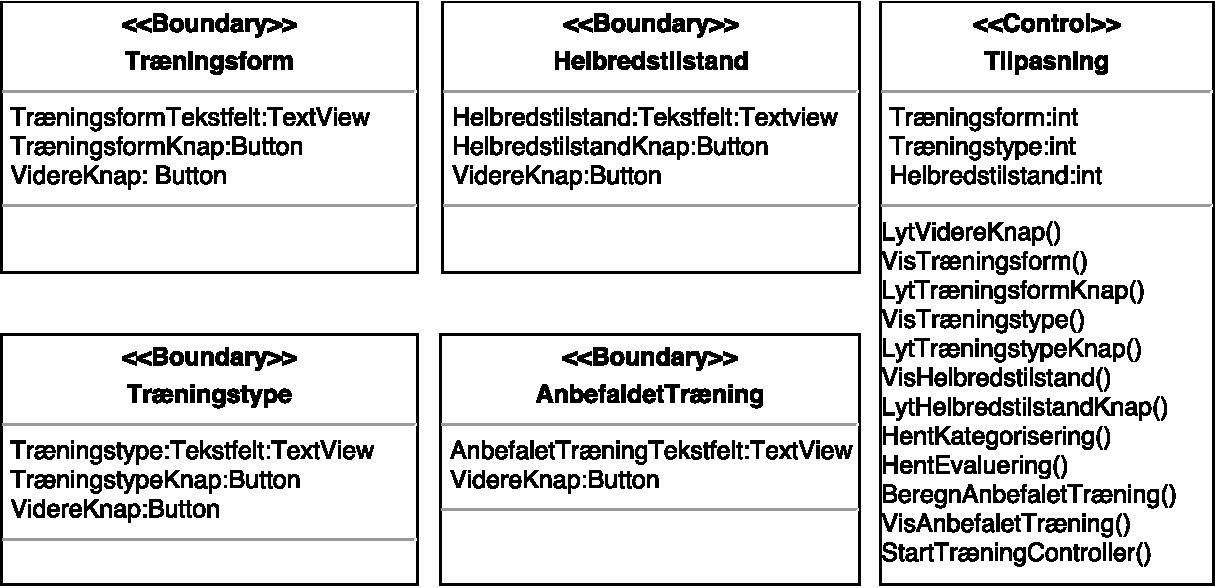
\includegraphics[width=0.9\textwidth]{figures/MVC/MVCTilpasning}
\caption{Designklasser for tilpasning af træningsniveau.}
\label{fig:DesignTilpasning}
\end{figure}

Der er opstilles fire grænseflader for henholdsvis \textit{TræningsformGrænseflade}, \textit{TræningstypeGrænseflade}, \textit{HelbredstilstandGrænseflade} og \textit{AnbefaldetTræningGrænseflade}. Dette er valgt, da det ønskes at gøre app’en overskuelig samt brugervenlig. Hertil skal brugeren foretage minimale valg på hver brugergrænseflade, således brugeren ikke eksponeres til for mange valg samt informationer. 
Den første grænseflade som vises er \textit{TræningsformGrænseflade}. Denne grænseflade indeholder et tekstfelt, der beskriver, hvad brugeren skal angive. Dertil er der opstillet tre knapper, af typen button, til valg af konditionstræning, styrketræning eller vejrtrækningsøvelser. Der forekommer ligeledes en tilbage- samt videreknap. Tilbageknappen tillader brugeren at returnere til hovedmenuen, der ses af \autoref{sec:MVCHovedmenu}. Videreknappen benyttes for at indikere, at brugeren har valgt den ønskede træningform, og kan derved kun benyttes, hvis en træningsform er valgt. 
Efterfølgende vises \textit{TræningstypeGrænseflade}, der indeholder et tekstfelt, som igen beskriver, hvad brugeren skal angive. Tre knapper er hertil opstillet, disse knapper tilhører træningstype 1, 2 eller 3. I denne grænseflade ses ligeledes en tilbage- samt videreknap. Tilbageknappen giver i denne anledning brugeren mulighed for at returnere tilbage til  foregående valg om den ønskede træningsform. Videreknappen fungerer igen ved at indikere, at brugeren har valgt den ønskede træningstype, og kan derfor kun benyttes, hvis træningstypen er valgt. 
Helbredstilstanden skal herefter angives, hvilket fremgår i \textit{HelbredstilstandGrænseflade}. Denne grænseflade består af et tekstfelt, der informerer brugeren om den daglige helbredstilstand, samt fem knapper, af typen button, til angivelse af brugerens tilstand. Derudover findes der ligeledes en tilbageknap, der henviser tilbage til \textit{TræningstypeGrænsefladen}, samt en videreknap, der igen indikerer, at brugeren har angivet sin helbredstilstand, og er klar til at fortsætte til træning. 
Efter træningsform samt type og den daglige helbredstilstand er angivet vises en \textit{AnbefaldetTræningGrænseflade}. Herunder forekommer tekstfelter, der oplyser den anbefalede træning samt tilsluttede kompatible måleenheder. Dertil opstilles en tilbageknap, der henviser tilbage til \textit{HelbredstilstandGrænseflade}, samt en startknap, som påbegynder træningen. 

Den tilhørende \textit{TilpasningAfTræningsniveauController} til de ovenstående boundarys lagrer den angivne træningsform, træningstype samt helbredstilstand, således disse senere kan benyttes til at beregne det passende træningsniveau. Controlleren reagerer på de forskellige angivelser af knapper fra de fire boundarys, hvortil angivelsen lagres idet brugeren benytter videreknappen, der henviser til den efterfølgende boundary. Foruden dette kan der ved tryk af tilbageknappen henvises til den foregående boundary. 
Controlleren henter endvidere brugerens individuelle kategorisering samt evaluering, der sammen med træningsform, træningstype og helbredstilstand udgør værdierne for beregningen af træningsniveauet. 

Da \textit{AnbefaldetTræningGrænseflade} indeholder et tekstfelt, der oplyser om tilkoblet kompatible måleenheder, forekommer endnu en controller til denne grænseflade. Denne ses af \autoref{fig:kompatiblemåleenheder}.

\begin{figure} [H]
\centering
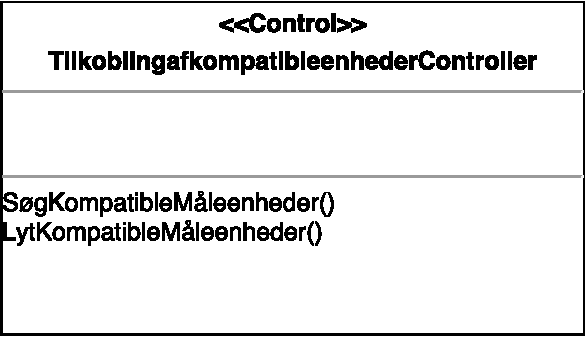
\includegraphics[width=0.9\textwidth]{figures/MVC/MVCKompMaale}
\caption{Designklasse for kompatible måleenheder.}
\label{fig:kompatiblemåleenheder}
\end{figure}

Tekstfeltet, hvori tilsluttet kompatible måleenheder oplyses styres af \textit{TilkoblingafkompatibleenhederController}, da det er denne som får informationen af den kompatible måleenhed.
\textit{TilkoblingafkompatibleenhederController} håndterer kommunikationen mellem systemet og de kompatible måleenheder. Controlleren tilgås ikke af brugeren, da det ønskes, at denne er en autonom funktion, der søger efter kompatible måleenheder førend en træning påbegyndes. Hertil har controlleren metoder til at søge efter enheder og hente målingerne de foretager.

